\directlua{includeCode("hazardous/nfpa")}

\definecolor{nfpaFire}      {RGB}{255, 102, 102}
\definecolor{nfpaHealth}    {RGB}{102, 145, 255}
\definecolor{nfpaReaction}  {RGB}{252, 255, 102}
\definecolor{nfpaOther}     {RGB}{252, 255, 255}

% official
\def\nfpaAsphyxiant{\Large SA}
\def\nfpaNoWater{\LARGE\Sout[2pt]{\hspace{0.1em}W\hspace{0.1em}}}
\def\nfpaOxidiser{\Large OX}

% inofficial
\def\nfpaAcid{\large ACID}
\def\nfpaAlkaline{\large ALK}
\def\nfpaBioHazard{\Huge\DejaVuSans^^^^2623}
\def\nfpaCorrosive{\large COR}
\def\nfpaCryogenic{\Huge\DejaVuSans^^^^2744}
\def\nfpaEcoHazard
{%
  \begin{tikzpicture}%
    \node [ white ] at  ( 0,  0 ) {\large ECO};
    \node           at  ( 0,  0 ) {
\includegraphics[height=1.5em]{\source/assets/pictograms/other/ecoHazard.pdf}};
  \end{tikzpicture}%
}
\def\nfpaEtching
{%
  \begin{tikzpicture}%
    \node [ white ] at  ( 0,  0 ) {\large COR};
    \node           at  ( 0,  0 ) {
\includegraphics[height=1em]{\source/assets/pictograms/other/corrosive.pdf}};
  \end{tikzpicture}%
}
\def\nfpaExplosive
{%
  \begin{tikzpicture}%
    \node [ white ] at  ( 0,  0 ) {\large EXP};
    \node           at  ( 0,  0 ) {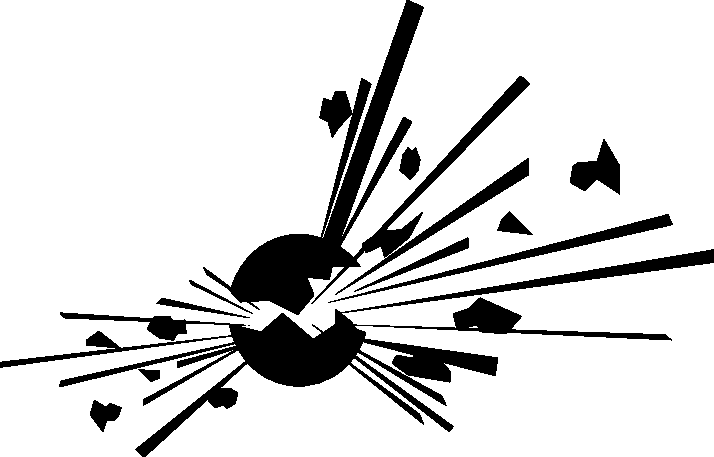
\includegraphics[height=1.5em]{\source/assets/pictograms/other/explosive.pdf}};
  \end{tikzpicture}%
}
\def\nfpaHot{\LARGE\FontAwesomeSolid^^^^f2c8}
\def\nfpaRadioactiv{\radioactivity}
\def\nfpaToxic{\Huge\DejaVuSans^^^^2620}

\newcommand{\nfpaDiamond}[5][2cm]
{%
  % 1 – size
  % 2 – fire hazars
  % 3 – health hazards
  % 4 – reaction hazards
  % 5 – other hazards
  \resizebox{#1}{!}%
  {%
    \begin{tikzpicture}[rotate=225]%
      \contourlength{0.05em}%
      \fill [ nfpaFire      ] ( 0,  0 ) rectangle ( 1,  1 );%
      \fill [ nfpaHealth    ] ( 1,  0 ) rectangle ( 2,  1 );%
      \fill [ nfpaReaction  ] ( 0,  1 ) rectangle ( 1,  2 );%
      \fill [ nfpaOther     ] ( 1,  1 ) rectangle ( 2,  2 );%
      \draw ( 0,  2 ) grid  ( 2,  0 );%
      \node at  ( 0.5,  0.5 ) {\contour{nfpaOther}{\huge#2}};%
      \node at  ( 1.5,  0.5 ) {\contour{nfpaOther}{\huge#3}};%
      \node at  ( 0.5,  1.5 ) {\contour{nfpaOther}{\huge#4}};%
      \node at  ( 1.5,  1.5 ) {#5};%
    \end{tikzpicture}\relax%
  }%
}
